\documentclass{beamer}

\usetheme{Copenhagen}
\usepackage[utf8]{inputenc}
\usepackage{graphics}

% Slayt basliklarinda kullanilan font boyutu
\setbeamerfont{frametitle}{size=\normalsize}

\title{Geometric Constraints for Human Detection in Aerial Imagery}
\author{Vladimir Reilly, Berkan Solmaz, Mubarak Shah}
\date{2010}
\institute[CVL]{Computer Vision Lab, University of Central Florida, Orlando,
USA}

\begin{document}

\frame{\titlepage}

\section[İskelet]{}
\frame{\tableofcontents}

\frame {
	\frametitle{Özet}

	\begin{itemize}
		\item UAV görüntülerde insanları algılamak
		\item hedef, çok az sayıda piksel barındırır
		\item Bu çalışmada görüntüye ek olarak \textbf{metadata} kullanıldı
		\item zemin normali ve insan gölgesinin yönelimi bellidir
		\item gölge yönelimini otomatik belirleyecek yöntem de önerildi
		\item buradaki yöntem \textbf{tek} kare temellidir
		\item wavelet öznitelik kombinasyonu ve SVM kullanıldı
		\item VIVID dataseti kullanılmıştır
	\end{itemize}

}

\section{Giriş}

\frame {
	\frametitle{UAV}

	\begin{block}{UAV}
		Unmanned Aerial Vehicle
	\end{block}

	\begin{itemize}
		\item gözetim (surveillance), askeri, güvenlik
		\item detection, tracking, classification ve event analysis
		\item yakın zamana ait havadan detecting-tracking ile alakalı
 		      cite{cheng06} ve cite{xiao08} çalışmalar insanı algılayamaz
		\item yerdeyken ki çekimlerden insan analiziyle ilgili tonlarca çalışma
		      yapılmıştır: cite{dalal05}, cite{felzenswalb08}, cite{leibe05},
			  cite{mikolajczyk04} ve cite{sabzmeydani07}
	\end{itemize}
}

\frame {
	\frametitle{yerden X gökten}

	\begin{itemize}
		\item \textbf{yerden} olanlarda insan $128x64$ gibi büyük boyutludur (ör. INRIA
			  dataseti)
		\item ve karşı cepheden görür
		\item \textbf{gökten} olanlarda insan $24x14$ gibi çok küçüktür ve
			  görünür parçası yoktur
		\item yerden olanlara uygulanan yöntemler geçersiz olur
		\item havai makinenin hareketi dolayısıyla yönelim açısından çok büyük
			  varyasyona sahiptir
		\item ayırt edici özellikler siliktir, bu yüzden false detection oranı
			  yüksektir
		\item "Person Tracking in UAV video" @ cite{xiao07} ve cite{miller07}
	\end{itemize}
}

\frame {
	\frametitle {İlgili Makaleler}

	\begin{itemize}
		\item cite{xiao07} ve cite{bose04}, hareket bilgisini kullandı
		\item hareket eden nesneler Histogram of oriented gradients
			  (\textbf{HOG}: cite{dalal05}) + SVM yardımıyla sınıflandı
		\item insan durağansa? gölge olduğunda? bloblar birbirine benzer takip
			  güçleşir
	\end{itemize}

}

\frame {
	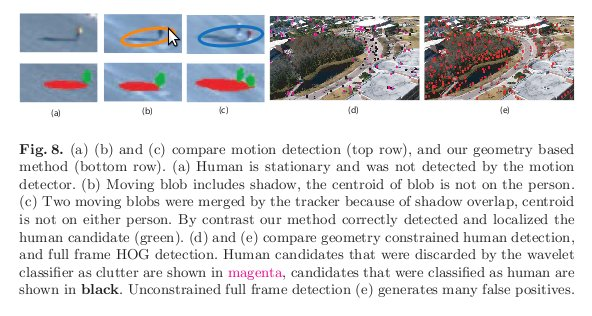
\includegraphics[width=1.0\textwidth]{img/fig8.jpg}
}

\frame {
	\frametitle {İlgili Makaleler}

	cite{miller07}

	\begin{itemize}
		\item Harris corner özniteliğini kullanmıştır
		\item daha sonra OT-MATCH filtreden geçirilir
		\item insanı şekillendiren nokta sayısı çok fazladır
	\end{itemize}
}

\frame {
	\frametitle {Makalenin Yaklaşımı}

	\begin{itemize}
		\item UAV platformundan elde edilen metadata:
		\item yerin normali ki insanın yönelimini verir
		\item önce gölge bulunur (daha fazla alanı kaplıyor)
		\item burada insanın yüksekliği ve gölge uzunluğu kullanılarak
		\item insan adaylarından wavelet öznitelikleri çıkarılır: geometrik
			  kısıtlama yaklaşımı
		\item SVM ile insan veya değil şeklinde sınıflandırılır
	\end{itemize}
}

\frame {
	\frametitle{Üstünlükleri}

	\begin{itemize}
		\item motion detection gereksizdir
		\item güçlü gölgeler performansı etkilemez
	\end{itemize}
}

\frame {
	\frametitle{Metadata}

	\begin{itemize}
		\item metadata yoksa, statik görüntüden gölge bulucular kullanılabilir
	\end{itemize}
}

\frame {
	\frametitle {}

	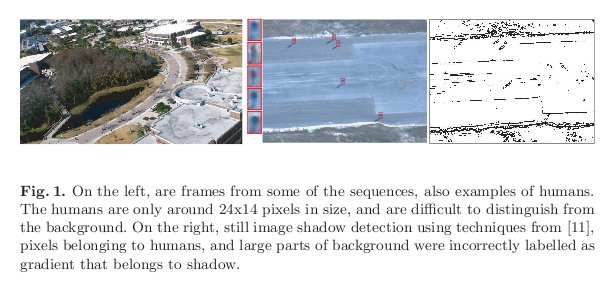
\includegraphics[width=1.0\textwidth]{img/fig1.jpg}
}

\section{Ground-Plane Normal and Shadow Constraints}

\subsection{Metadata}

\frame {
	\frametitle{Metadata}

	\begin{itemize}
		\item latitude, longitude, altitude parametrelerini içerir
		\item pitch, yaw, roll hesaplanabilir
		\item ayrıca kamera parametreleri: scan, elevation, twist (uçağa göre
			  değişimler), focal length, time
		\item dünyayla ilgili kısıtları belirler
	\end{itemize}
}

\subsection{World Constraints}

\frame {
	\frametitle{World Constraints}

	\begin{itemize}
		\item nesne algılama ve gözetim senaryolarında genelde gürültü olarak görülür
		\item havadan gözlem durumunda ise nesnenin kendisine ait bilginin
			  yetersizliğini tolere etmede kullanılır
		\item Kısıtlar şunlardır:
		\item kişi yeryüzeyine göre diktir
		\item kişinin gölgesi vardır
		\item kişinin yüksekliğiyle gölgesinin uzunluğu arasında geometrik
		ilişki vardır
	\end{itemize}
}

\frame {
	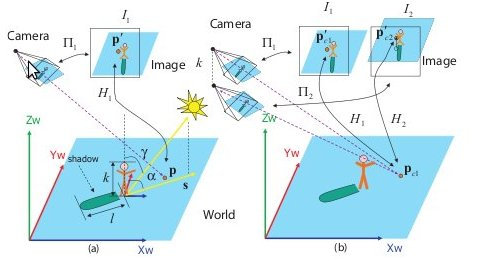
\includegraphics[width=0.8\textwidth]{img/fig2.jpg}
}

\subsection{Image Constraints}

\section{Human Detection}
\subsection{Constraining the Search}
\subsection{Exploiting Object Shadow Relationship}
\subsection{Constraints without Metadata}
\subsection{Object Candidate Classification}

\section{Results}

\section{Conclusions}

\end{document}
